\subsection{CMB temperature anisotropies: multipoles}\label{sec:CMBMultipoles}
The temperature anisotropy in the $\mathbf{n}$ direction in the sky is a square-integrable function on the sphere and thus can be expanded in terms of spherical harmonics
\begin{eqopt}[darkred]\label{eq:harmonicExpansion}
    \frac{\delta T_{now}}{T_{now}}(\mathbf{n}) = \sum_{l=1}^\infty\sum_{m=-l}^{l} a_{lm}Y_{lm}(\mathbf{n})
\end{eqopt}
Using common conventions, we introduce spherical harmonics and (associated) Legendre polinomials as follows:
\begin{eqopt}[darkgreen]
    Y_{l}^m(\theta ,\varphi)=(-1)^m \sqrt{\frac{2l+1}{4\pi} \frac{(l-m)!}{(l+m)!}}\,e^{im\phi}\,P_{l}^m(\cos{\theta}) \qquad P_{l}^{-m} = (-1)^m\frac{(l-m)!}{(l+m)!} P_{l}^{m}
\end{eqopt}
It follows that $ {Y_{l}^m}^* = (-1)^m Y_{l}^{-m}$ and, from~\eqref{eq:harmonicExpansion}, $a^*_{lm}=(-1)^m a_{l-m}$. It also follows that
\begin{eqopt}[darkred]
    \int_0^{\pi} d\theta \int_{0}^{2\pi}  Y_{l}^m Y_{l'}^{-m'} sin(\theta) d\theta d\phi = \delta_{ll'} \delta_{mm'}
\end{eqopt}
We can use this orthonormality to determine the \textit{multipole moments} $a_{lm}$:
\begin{equation}
    a_{lm}=\int d\mathbf{n} \frac{\delta T_{now}}{T_{now}}(\mathbf{n}) Y^*_{lm}(\mathbf{n})
\end{equation}

The CMB \textit{angular power spectrum} $C_l$ we obtain experimentally is the ensemble two-point function of the $a_{lm}$.  One then considers an average over all possible realizations of the Universe (a hypothetical average over infinitely many CMB skies)\footnote{Not to be confused with the inner product on the 2-sphere, which decomposes \emph{one} sky map into modes.}
\begin{equation}\label{eq:ensembleAverage}
    \bigl<a_{lm}a^*_{l'm'} \bigr>=C_l \,\delta_{ll'}\,\delta_{mm'} \qquad \hat{C}_l = \frac{1}{2l+1} \sum_{m=-l}^l \abs{a_{lm}}^2 \approx C_l
\end{equation}
The introduction of an \textit{estimator} $\hat{C}_l$ for $C_l$ is motivated due to the fact that, for fixed $l$, we have $2l+1$ different $a_{lm}$, allowing for $2l+1$ independent estimated of $C_l$.
Because the process is assumed statistically isotropic, all the $2l+1$ different $m$-modes at fixed $l$ are statistically equivalent, hence averaging over them in our one sky gives an unbiased estimator of the ensemble-average power~\cite{CosmologyBau}.
$\hat{C}_l = C_l$ in the infinite ensemble limit, i.e.\ $\bigl<\hat{C}_l \bigr>=C_l$. However, we have a nonzero \textit{cosmic variance}
\begin{eqopt}[darkred]
    \frac{\Delta C_l}{C_l}= \sqrt{\frac{2}{2l+1}}
\end{eqopt}
which can be proved using Wick's theorem in quite a long calculation starting from $\Delta C_l \equiv \sqrt{\bigl<(C_l-\hat{C}_l)^2 \bigr>}$ . We thus have large errors for small $l$ values.
\begin{comment}
If you look at a single $l$ pattern on the sky, you'll see alternating rings (for $m =0$) or lobes (for $m \neq0$).
The Legendre polinomials $P_l^0 (\cos{\theta})$ have exactly $l$ zeros in the interval $0,\pi$, the first one is $\theta \sim \pi /2l$, a full oscillation of the pattern (hot $\rightarrow$ cold $\rightarrow$ hot) on the sphere takes two of those zero-crossings, i.e.\ an angular period $\Delta \theta \sim \pi/l$.
Therefore, for large $l$, a multipole $l$ corresponds to a small angular scale and statistics gets better (as sample scales as $2l+1$).
\end{comment}
 
The CMB temperature fluctuations are analyzed statistically by measuring the correlations
between hot and cold spots as a function of their angular separation.
\begin{figure}[h]
      \centering
        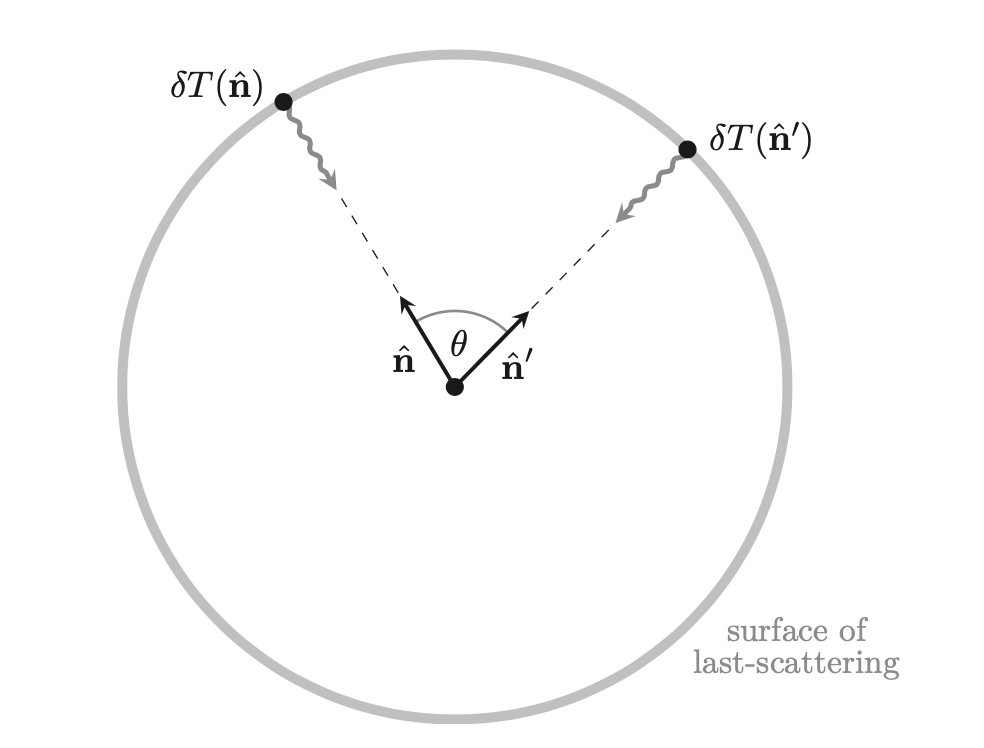
\includegraphics[width=0.8\textwidth]{Graphics/CMB-2point.png}
        \caption{2-point correlations $\bigl<\frac{\delta T}{T} (\mathbf{n})\frac{\delta T}{T} (\mathbf{n}')\bigr>$ between temperature fluctuations on LSS~\cite{CosmologyBau}.}
  \end{figure}
  Employing the \textit{addition theorem},
  \begin{eqopt}[darkred]\label{eq:additionTh}
     \sum_{m=-l}^l Y^m_l(\mathbf{n}){Y^m_l}^*(\mathbf{n}') = \frac{2l+1}{4\pi} P_l Y^m_l(\mathbf{n}\cdot\mathbf{n}')
  \end{eqopt}  
  It is easy to show that 
  \begin{equation}
    \bigl<\frac{\delta T}{T} (\mathbf{n})\frac{\delta T}{T} (\mathbf{n}')\bigr> = \sum_{ll'}\sum_{mm'}\bigl<a_{lm}a_{l'm'}^* \bigr>Y^m_l(\mathbf{n}) Y^{m'}_{l'}(\mathbf{n}') =\sum_l C_l \frac{2l+1}{4\pi} P_l(\mathbf{n}\cdot\mathbf{n}')
  \end{equation}
  For large $l$, setting $\mathbf{n} = \mathbf{n}'$ $(P_l(1)=1 \quad \forall\, l)$,
  \begin{equation}
  \bigl<\frac{\delta T}{T} (\mathbf{n})\frac{\delta T}{T} (\mathbf{n}')\bigr> \approx \int d\log{l} \frac{l^2+1}{2\pi}C_l
  \end{equation}
  One usually plots the CMB power spectrum as
  \begin{eqopt}[darkgreen]
    \mathcal{D}_l \equiv T_0^2 \frac{l(l+1)}{2\pi}C_l
  \end{eqopt}
  \vspace{-0.6cm}
  
  We now want to express the angular power spectrum in terms of perturbations during inflation.
  Using~\eqref{eq:ensembleAverage}~\eqref{eq:harmonicExpansion}~\eqref{eq:additionTh} we get 
  \begin{equation}
    C_l =\frac{1}{4\pi} \int d\mathbf{n} d\mathbf{n}' \bigl<\frac{\delta T}{T} (\mathbf{n})\frac{\delta T}{T}^* (\mathbf{n}')\bigr> P_l(\mathbf{n}\cdot\mathbf{n}')
  \end{equation}
  Then \underline{assume instantaneous recombination}, i.e.\ infinitely small LSS, and expand $\frac{\delta T}{T}$ in Fourier space with a further expansion of a plane wave in terms of Legendre polinomials. A rather technical derivation brings to
\begin{eqopt}
    C_l = \frac{2}{\pi}\int dk k^2 P_{\Phi}(k) \underbracket{\tilde{\frac{\delta T}{T}}(k) \tilde{\frac{\delta T}{T}}^*(k) \left[j_l(k r_*)\right]^2}_{\text{transfer function}}
\end{eqopt}
where $ P_{\Phi}(k) \delta^{(3)}(\mathbf{k}+\mathbf{k}')\equiv \bigl<\Phi(\mathbf{k}) \Phi^*(\mathbf{k}') \bigr> $ is a primordial spectrum contribution coming from the power spectrum of scalar perturbations at recombination, while $\tilde{\frac{\delta T}{T}}(k)$ is defined to be independent of the gravitational field: $\frac{\delta T}{T} = \tilde{\frac{\delta T}{T}} \Phi$; $j_l$ is a spherical Bessel function ($r_*$ is the comoving radial distance from us to LSS).
The transfer function is determined by~\eqref{eq:SachsWolfe}.